\documentclass{standalone}
\makeatletter\AtBeginDocument{\@buildstepset{1,2,3,4}}\makeatother
\usepackage{tikz}
\usetikzlibrary{intersections, calc}
\usepackage{hsbcommon}
\begin{document}
    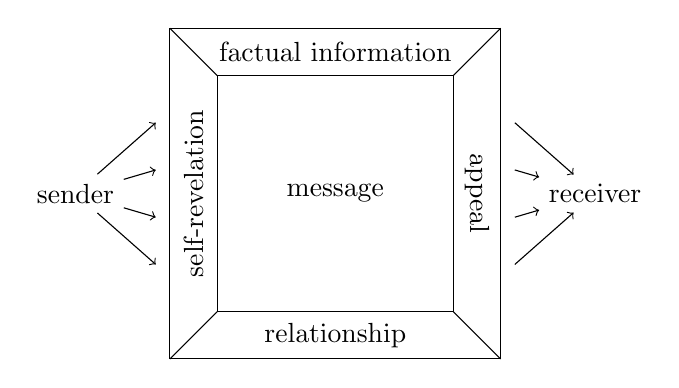
\begin{tikzpicture}[scale=0.6]
        \draw (0,0) rectangle (7,7);
        \draw (1,1) rectangle (6,6);
        \draw (1,1) -- (0,0);
        \draw (6,6) -- (7,7);
        \draw (6,1) -- (7,0);
        \draw (1,6) -- (0,7);
        \node at (3.5,3.5) {message};
        \node at (3.5,6.5) {factual information};
        \node[rotate=90] at (0.5,3.5) {self-revelation};
        \node[rotate=-90] at (6.5,3.5) {appeal};
        \node at (3.5,0.5) {relationship};
        \node (S) at (-2,3.5) {sender};
        \node (R) at (9,3.5) {receiver};
        \foreach \i in {5,4,3,2} {
            \draw[->] (S) -- (-0.3,\i);
            \draw[->] (7.3,\i) -- (R);
        };
    \end{tikzpicture}
\end{document}